\documentclass{article} % say
\usepackage{tikz}
\usetikzlibrary{arrows,decorations.pathmorphing,backgrounds,positioning,fit}
\begin{document}
\begin{tikzpicture}
  \draw (0,0) -- (1,1);
\end{tikzpicture}

\vspace{1cm}

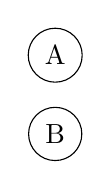
\begin{tikzpicture}
\path 
	(0,2) node [shape=circle,draw]{A}
	(0,1) node [shape=circle,draw]{B};
\end{tikzpicture}

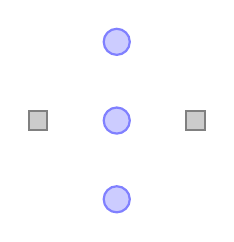
\begin{tikzpicture}[thick]
  \node at ( 0,2) [circle,draw=blue!50,fill=blue!20] {};
  \node at ( 0,1) [circle,draw=blue!50,fill=blue!20] {};
  \node at ( 0,0) [circle,draw=blue!50,fill=blue!20] {};
  \node at ( 1,1) [rectangle,draw=black!50,fill=black!20] {};
  \node at (-1,1) [rectangle,draw=black!50,fill=black!20] {};
\end{tikzpicture}

\tikzset{
place/.style={circle,draw=blue!50,fill=blue!20,thick,
                  inner sep=0pt,minimum size=6mm},
   transition/.style={rectangle,draw=black!50,fill=black!20,thick,
                       inner sep=0pt,minimum size=4mm}
}

\vspace {1cm}
\begin{tikzpicture}
  \node at ( 0,2) [place] {};
  \node at ( 0,1) [place] {};
  \node at ( 0,0) [place] {};
  \node at ( 1,1) [transition] {};
  \node at (-1,1) [transition] {};
\end{tikzpicture}


\vspace {1cm}
\begin{tikzpicture}
  \node[place]      (waiting)                            {};
  \node[place]      (critical)       [below=of waiting]  {};
  \node[place]      (semaphore)      [below=of critical] {};
  \node[transition] (leave critical) [right=of critical] {};
  \node[transition] (enter critical) [left=of critical]  {};
  \node [red,above] at (semaphore.north) {$s\le 3$};
\end{tikzpicture}


\vspace {1cm}
\begin{tikzpicture}[every label/.style={red}]
  \node[place]      (waiting)                            {};
  \node[place]      (critical)       [below=of waiting] {};
  \node[place]      (semaphore)      [below=of critical,
                                      label=above:$s\le3$] {};
  \node[transition] (leave critical) [right=of critical] {};
  \node[transition] (enter critical) [left=of critical] {};
\end{tikzpicture}

% With arrows
\vspace{1cm}
\begin{tikzpicture}
  \node[place]      (waiting)                            {};
  \node[place]      (critical)       [below=of waiting]  {};
  \node[place]      (semaphore)      [below=of critical] {};
  \node[transition] (leave critical) [right=of critical] {};
  \node[transition] (enter critical) [left=of critical]  {};
  \draw [->] (critical.west) -- (enter critical.east);
\end{tikzpicture}

\vspace{1cm}
\begin{tikzpicture}
  \node[place]      (waiting)                            {};
  \node[place]      (critical)       [below=of waiting] {};
  \node[place]      (semaphore)      [below=of critical] {};
  \node[transition] (leave critical) [right=of critical] {};
  \node[transition] (enter critical) [left=of critical] {};
  \draw [->] (enter critical) to                 (critical);
  \draw [->] (waiting)        to [bend right=45] (enter critical);
  \draw [->] (enter critical) to [bend right=45] (semaphore);
\end{tikzpicture}


\vspace{1cm}
\begin{tikzpicture}
  \node[place]      (waiting)                            {};
  \node[place]      (critical)       [below=of waiting] {};
  \node[place]      (semaphore)      [below=of critical] {};
  \node[transition] (leave critical) [right=of critical] {};
  \node[transition] (enter critical) [left=of critical] {};
  \draw [->] (enter critical) to                 (critical);
  \draw [->] (waiting)        to [out=135,in=90] (enter critical);
\end{tikzpicture}


%%%%%%%%%%%%%%%%%%%%%%%%%%%%%%%%%%%%5
\vspace{1cm}
This is a cool way of making edges
\begin{tikzpicture}
  \node[place]      (waiting)                            {};
  \node[place]      (critical)       [below=of waiting]  {};
  \node[place]      (semaphore)      [below=of critical] {};
  \node[transition] (leave critical) [right=of critical] {};
  \node[transition] (enter critical) [left=of critical]  {EC}
    edge [->]               (critical)
    edge [<-,bend left=45,red] (waiting)
    edge [->,bend right=45] (semaphore);
\end{tikzpicture}

\vspace{1cm}
My own stuff
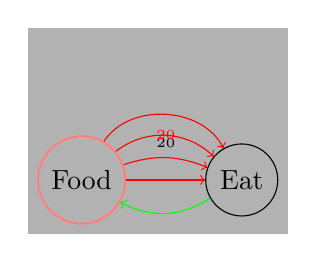
\begin{tikzpicture}
\node[draw=black!30] (dingo) {                    };
\node[circle,draw=red!50,thick] (food)[below=of dingo] {Food};
\node[circle,draw,] (eat) [right=of food] {Eat}
	edge [<-,bend right=0, red]  (food)
	edge [<-,bend right=20, red] node[auto,swap,black] {\tiny 20} (food)
	edge  [<-,bend right=40, red] node {\tiny 20} (food)
	edge [<-,bend right=60, red] (food)
	edge [->,bend left, green] (food);

\begin{pgfonlayer}{background}
\node [fill=black!30,fit=(dingo) (food) (eat)] {};
\end{pgfonlayer}

\end{tikzpicture}

\end{document}

